\documentclass{beamer}

%%%%%%%%%%%%%%%%%%%%%%%%%%%%%%%%%%
% PAKCAGES
%%%%%%%%%%%%%%%%%%%%%%%%%%%%%%%%%%

\usepackage{etoolbox}
\usepackage{xparse}
\usepackage{graphicx}
\usepackage{subcaption}
\usepackage{moresize}
\usepackage{anyfontsize}

\usepackage{calculator}



\makeatletter

\NewDocumentCommand{\setFontSize}{m o m}{%
    \IfNoValueF{#2}{%
        \fontsize{#1}{#2}\selectfont#3%
    }{%
        % see https://texblog.org/2012/08/29/changing-the-font-size-in-latex/
        \MULTIPLY{#1}{1.2}{\setFont@baseline}%
        \fontsize{#1}{\setFont@baseline}\selectfont#3%
    }%
}

\NewDocumentCommand{\todo}{m}{%
    {\color{blue} #1}%
}

\NewDocumentCommand{\code}{m}{%
    \texttt{#1}%
}

\makeatother
\NewDocumentCommand{\CPD}{}{%
    \texttt{CPD}%
}

\NewDocumentCommand{\ALT}{}{%
    \texttt{ALT}%
}

\NewDocumentCommand{\AWA}{}{%
    \texttt{AWA$^*$}%
}

\NewDocumentCommand{\WA}{}{%
    \texttt{WA$^*$}%
}

\NewDocumentCommand{\A}{}{%
    \texttt{A$^*$}%
}

\NewDocumentCommand{\CPDSearch}{}{%
    \texttt{CPD-Search}%
}

\NewDocumentCommand{\anytimeCPDSearch}{}{%
    \texttt{Anytime CPD-Search}%
}


\NewDocumentCommand{\CPDPathName}{}{%
    \texttt{CPD}-Path%
}

\NewDocumentCommand{\CPDPathsName}{}{%
    \texttt{CPD}-Paths%
}

\NewDocumentCommand{\CPDPath}{m m}{%
    \texttt{CPD-Path}[#1, #2]%
}

\NewDocumentCommand{\CPDPathCostOriginal}{m m}{%
    \ifmmode{h_{CPD}[#1]}\else{$h_{CPD}[#1]$}\fi%
}

\NewDocumentCommand{\CPDPathCostNew}{m m}{%
    \ifmmode{h'_{CPD}[#1]}\else{$h'_{CPD}[#1]$}\fi%
}

\NewDocumentCommand{\pathOnGraph}{m m}{%
    path[#1, #2]%
}

\NewDocumentCommand{\pathCostOnGraph}{m m}{%
    cost(path[#1, #2])%
}


\usetheme{Frankfurt}

\title{Path Planning with CPD Heuristics}
%\subtitle{}

\author{Massimo Bono$^1$, Alfonso E. Gerevini$^1$, Daniel D. Harabor$^2$ and Peter J.Stuckey$^2$}
\institute{%
    $^1$\setFontSize{7.8}{Dipartimento di Ingegneria dell'Informazione, Università degli Studi di Brescia, Italy}%
    \\%
    $^2$\setFontSize{7.8}{Faculty of Information Technology, Monash University, Melbourne, Australia}%
    \\%
    \{mbono, alfonso.gerevini\}@unibs.it, \{daniel.harabor, peter.stuckey\}@monash.edu%
}
%\date{\today}
\date{August 15, 2019}

\setInputPath{%
    {src/texs}%
    {src/images}%
    {src/tikzs}%
    {src/bibs}%
}

\begin{document}

%https://stackoverflow.com/a/3210406/1887602
\beamertemplatenavigationsymbolsempty

% tempo totale: 13 minuti => 50 secondi per slide! è chiaro che qualche slide va rimossa
% High level
% SLIDE 1: titolo
% SLIDE 2: 
%    - path finding è importante (videogiochi, routing); moderne soluzioni usano auxiliary data per calcolare velocemente;
%    - una variante del problema è quella in cui i costi degli archi non sono fissi, ma cambiano. 
%    - data una mappa, dopo che delle perturbazioni non decrescenti l'hanno modificata, come possiamo calcolare velocemente il percorso ottimo?
%    - quest apresentazione cercherà di rispondere a questa domanda.
% SLIDE 3: 
%   - esempio per motivare il lavoro: siamo su una mappa stradale e stiamo seguendo un percorso ottimo. Ad un certo punto
% sul nostro percorso ottimo scopriamo che  c'è un ingorgo che ci rallenterebbe. Abbiamo quindi la scelta di:
% ricalcolare il nostro percorso ottimo da zero sulla nuova mappa (mappa originale + perturbazioni) oppure possiamo
% cercare di calcolare il percorso ottimo sfruttando le informazioni precedenti (mappa originale senza perturbazioni)
% SLIDE 4: table of contents
%   context and background: CPD, ALT, AWA*
%   proposed technique:
%       - CPD Search
%       - Anytime CPD Search
%   Experimental results:
%       - optimal;
%       - anytime;
%   Conclusions and future works;
% SLIDE 5: secondo me qui è meglio scrivere bene il nostro context (ovvero perturbazioni online, preprocessing offline) dato
%   che è stato un punto che ha creato criticità nella rebuttal;
%   - il tempo di prerocessing offline non deve essere ammortizzato nell'online;
% SLIDE 6: CPD (citazione)
%   - esempio di costruzione (per intenderci quello con la mappa 3x3, non quello di Harabor nel paper);
%   - esempio di matrice delle adiacenze => compressione con un mini esempio;
%   - esempio di query, come si fa inserendo la complessità (da s -> a, da a->b, da b -> g);
% SLIDE 7: ALT (citazione)
%   - disuguaglianza triangolare con il massimo;
%   - Dico come abbiamo fatto a posizionare i landmark;
% SLIDE 8: AWA* (citazione)
%   - Idea: usare le soluzione trovate per fare pruning sulla ricerca;
% SLIDE 9: CPD-Search
%   - nodo di ricerca: location
%   - MAIN IDEAS:
%       * il percorso calcolato dal CPD nella mappa originale è un lowerbound del percorso ottimo calcolabile
%       nella mappa parturbata (siccome le perturbazioni sono non-decrescenti) => euristica ammissibile;
%       * dato una posizione s, se il percorso generato dal CPD (che è ottimo) è privo di perturbazioni possiamo terminare la ricerca e calcolare
%           immediatamente il percorso ottimo => early termination;
% SLIDE 10: sicuramente qui andrebbe messo qualcosa in più della "main idea". Il problema è che non voglio mettere l'algoritmo... troppo
% lungo e complesso da commmentare.
% SLIDE 11: Experimental setup
%   - map pool: Sturtevant;
%   - how we generated perturbations:
%       - random perturbations on 10% of edges of the map (3x the original cost);
%       - perturbation affecting a whole area on a location on the optimal path of a query (up to 4x the original cost);
% SLIDE 12:
%   - optimal search:
%       - results on the cactus plots (hrt201n, dustwallowkeys, mazes);
% SLIDE 13
%   - anytime search:
%       - results on hrt201n map;
% SLIDE 14: Conclusion and Future works
%   - we applied CPD technique in the context of dynamic edge-cost;
%   - we proposed the application in the optimal, bounded and anytime context;
%   - we have experimentally evaluated the techniques performances against ALT's and showed significant gains;
%   FUTURE WORKS:
%   - application of CPD over temporally changing edge-costs for deisgning admissible and unadmissible heuristics;
%   - application of CPD in the MAPF setting;
%   - dare l'idea sulle idee di harabor /idee di saetti?
%       
%          



\begin{frame}[plain]
    \titlepage
\end{frame}
\section*{Introduction}

\begin{frame}{Introduction}
    \begin{itemize}
        \item Single-agent shortest path planning: given a graph, compute a path from a start node $s$ to a goal $t$ whose cost is minimum;
        \item Modern algorithms use auxiliary data structures to improve performances
        
        \begin{center}
            however
        \end{center}
        
        When \textbf{edge costs are dynamic} such algorithms may fail due to invalid auxiliary data.

        \item \textbf{Goal}: Solve dynamic-cost single agent path planning problems by exploiting Compressed Path Database (CPD);
        \item \textbf{Results}: developed new bounded, optimal and anytime A* variants using CPD whose experimentally-evaluated performances show substantial gains over previous algorithms.
    \end{itemize}
\end{frame}

%see https://tex.stackexchange.com/a/208409/145331
\begin{frame}[fragile]{A simple example}
    \begin{center}
        \textbf{Original Map}\\
    \end{center}

    \begin{minipage}{0.5\textwidth}
        \begin{tikzpicture}
            \matrix[square matrix]{
                |[fill=black!0]| $s_{0,0}$   &|[fill=black!0]| $s_{0,1}$  &|[fill=black!40]| $s_{0,2}$  \\
                |[fill=black!60]| $s_{1,0}$   &|[fill=black!20]| $s_{1,1}$  &|[fill=black!0]| $s_{1,2}$  \\
                |[fill=black!0]| $s_{2,0}$   &|[fill=black]|  &|[fill=black!0]| $s_{2,2}$  \\
            };
        \end{tikzpicture}
        
        \begin{tabular}{clcl}
            \drawFilledSquare{black!0} & 1 &
            \drawFilledSquare{black!20} & 3 \\
            \drawFilledSquare{black!40} & 5 &
            \drawFilledSquare{black!60} & 7 \\
            \drawFilledSquare{black} & $\infty$ &
            & \\
        \end{tabular}
    \end{minipage}%
    \begin{minipage}{0.5\textwidth}
        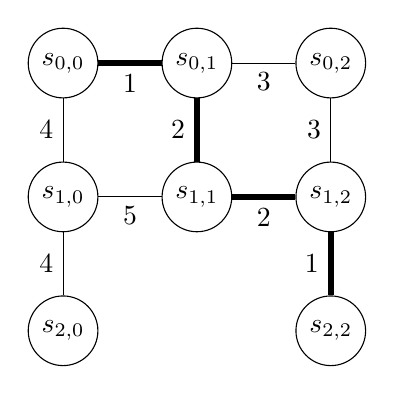
\begin{tikzpicture}
            \tikzset{Vertex/.style={%
                shape=circle,%
                draw=black,%
                minimum size=10pt,%
                radius=1cm,%
                inner sep=3pt,%
                node distance=1.7cm,%
            }}
    
            \node[Vertex] (v00) at (0,0) {$s_{0,0}$};
            \node[Vertex, right of=v00] (v01) {$s_{0,1}$};
            \node[Vertex, right of=v01] (v02) {$s_{0,2}$};
            \node[Vertex, below of=v00] (v10) {$s_{1,0}$};
            \node[Vertex, right of=v10] (v11) {$s_{1,1}$};
            \node[Vertex, right of=v11] (v12) {$s_{1,2}$};
            \node[Vertex, below of=v10] (v20) {$s_{2,0}$};
            \node[Vertex, below of=v12] (v22) {$s_{2,2}$};
    
            \path (v00) edge[-.,line width=2pt] node[below]{1} (v01);
            \path (v01) edge[-.] node[below]{3} (v02);
            \path (v10) edge[-.] node[below]{5} (v11);
            \path (v11) edge[-.,line width=2pt] node[below]{2} (v12);
            \path (v00) edge[-.] node[left]{4} (v10);
            \path (v10) edge[-.] node[left]{4} (v20);
            \path (v01) edge[-.,line width=2pt] node[left]{2} (v11);
            \path (v02) edge[-.] node[left]{3} (v12);
            \path (v12) edge[-.,line width=2pt] node[left]{1} (v22);
        \end{tikzpicture}
        $$s_{0,0} \rightarrow s_{0,1} \rightarrow s_{1,1} \rightarrow s_{1,2} \rightarrow s_{2,2}$$
    \end{minipage}
\end{frame}

\begin{frame}[fragile]{A simple example}
    \begin{center}
        \textbf{Perturbated Map}\\
    \end{center}

    \begin{minipage}{0.5\textwidth}
        \begin{tikzpicture}
            \matrix[square matrix]{
                |[fill=black!0]| $s_{0,0}$   &|[fill=black!0]| $s_{0,1}$  &|[fill=black!40]| $s_{0,2}$  \\
                |[fill=black!60]| $s_{1,0}$   &|[fill=black!60]| $s_{1,1}$  &|[fill=black!0]| $s_{1,2}$  \\
                |[fill=black!0]| $s_{2,0}$   &|[fill=black]|  &|[fill=black!0]| $s_{2,2}$  \\
            };
        \end{tikzpicture}
        
        \begin{tabular}{clcl}
            \drawFilledSquare{black!0} & 1 &
            \drawFilledSquare{black!20} & 3 \\
            \drawFilledSquare{black!40} & 5 &
            \drawFilledSquare{black!60} & 7 \\
            \drawFilledSquare{black} & $\infty$ &
            & \\
        \end{tabular}
    \end{minipage}%
    \begin{minipage}{0.5\textwidth}
        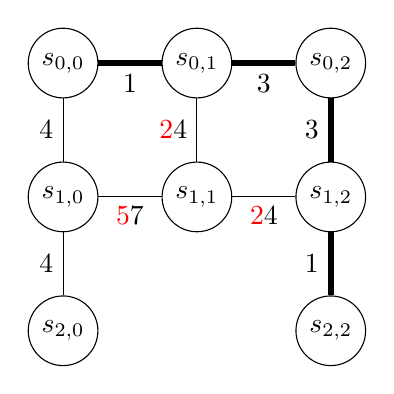
\begin{tikzpicture}
            \tikzset{Vertex/.style={%
                shape=circle,%
                draw=black,%
                minimum size=10pt,%
                radius=1cm,%
                inner sep=3pt,%
                node distance=1.7cm,%
            }}
    
            \node[Vertex] (v00) at (0,0) {$s_{0,0}$};
            \node[Vertex, right of=v00] (v01) {$s_{0,1}$};
            \node[Vertex, right of=v01] (v02) {$s_{0,2}$};
            \node[Vertex, below of=v00] (v10) {$s_{1,0}$};
            \node[Vertex, right of=v10] (v11) {$s_{1,1}$};
            \node[Vertex, right of=v11] (v12) {$s_{1,2}$};
            \node[Vertex, below of=v10] (v20) {$s_{2,0}$};
            \node[Vertex, below of=v12] (v22) {$s_{2,2}$};
    
            \path (v00) edge[-.,line width=2pt] node[below]{1} (v01);
            \path (v01) edge[-.,line width=2pt] node[below]{3} (v02);
            \path (v10) edge[-.] node[below]{{\color{red} \xcancel{5}}{7}} (v11);
            \path (v11) edge[-.] node[below]{{\color{red} \xcancel{2}}{4}} (v12);
            \path (v00) edge[-.] node[left]{4} (v10);
            \path (v10) edge[-.] node[left]{4} (v20);
            \path (v01) edge[-.] node[left]{{\color{red} \xcancel{2}}{4}} (v11);
            \path (v02) edge[-.,line width=2pt] node[left]{3} (v12);
            \path (v12) edge[-.,line width=2pt] node[left]{1} (v22);
        \end{tikzpicture}
        $$s_{0,0} \rightarrow s_{0,1} \rightarrow s_{0,2} \rightarrow s_{1,2} \rightarrow s_{2,2}$$
    \end{minipage}
\end{frame}

\begin{frame}{Talk Outline}
    \begin{itemize}
        \item Context and Background:
        \begin{itemize}
            \item Compress Path Database (\CPD{});
            \item \ALT{}, \AWA{};
        \end{itemize}
        \item Proposed Techniques: \CPDSearch{} and \anytimeCPDSearch{};
        \item Experimental Results: 
            \begin{itemize}
                \item optimal and 
                \item anytime scenario;
            \end{itemize}
        \item Conclusion and Future Work;
    \end{itemize}
\end{frame}


\end{document}
